\section{The Dedekind eta analogue at the basepoint one}\label{ch:bpeta}

At the basepoint one the pole of $\zeta$ and the primes act together: the pole term and the prime atoms of the L\'evy form both have infinite mass on $(1,\infty)$, the form converges only as a compensated limit, and quasi infinite divisibility is lost (Section~\ref{sb:sec:qid}). The $L$ function of the real character $\chi_{12}$ modulo $12$, to which Section~\ref{ch:chi12} carried the pipeline of the book, has no pole. Its completed function is entire and is a Mellin transform of the Dedekind eta function, whose product formula makes the kernel positive, and at the basepoint two its sine squared decomposition loses the pole piece while the prime weights take both signs (Section~\ref{sec:ch16:sin2}). We repeat for $L(s,\chi_{12})$ the calculations that Chapter~\ref{chap:basepoint} made for $\zeta$ at the basepoint one: the Thorin measure and the tail of the shifted clock (Section~\ref{bp:eta:sec}); the L\'evy form, its conversion by the sine squared lemma and its extension below the basepoint one, together with the question of Section~\ref{ch:sato} whether the tilted variable is quasi infinitely divisible (Section~\ref{bp:eta:sec:levy}); and the hitting time with its exact Brownian boundary (Section~\ref{bp:eta:sec:hit}). Together they redraw for $L(s,\chi_{12})$ the part of the map of Section~\ref{pm:sec:map} at the basepoint one.

Every step goes through with the same structure, and the constants change only through the denser zeros. The comparison of the two examples in Section~\ref{bp:sec:compare} therefore separates what in the example of $\zeta$ comes from the pole from what comes from the zeros, and it shows that removing the pole does not move the boundary of what is proved. The scripts are in the folder \texttt{basepoint\_one/eta} of the archive, and we name them at each table and figure.

\subsection{The completed \texorpdfstring{$L$}{L} function and its Thorin measure}\label{bp:eta:sec}

We use the completed function $\xi(s,\chi_{12})=(12/\pi)^{s/2}\Gamma(s/2)L(s,\chi_{12})$, its kernel $K$ and the variable $Y$ with density $K/\xi(\frac12,\chi_{12})$ of Section~\ref{sec:ch16:eta}; the function satisfies $\xi(s,\chi_{12})=\xi(1-s,\chi_{12})$ and is entire as it stands, with no factor like the $\frac12s(s-1)$ of $\xi$: $L(s,\chi_{12})$ has no pole to remove. We computed its zeros on the critical line by sign changes of $\xi(\frac12+it,\chi_{12})e^{\pi t/4}$ with \texttt{zeros12.py}, finding $297$ below height $340$; Section~\ref{sec:ch16:eta} lists the first of them. In this section $b_\alpha=(\xi'/\xi)(\alpha,\chi_{12})$ and $v_\alpha(\theta)=\re(\xi'/\xi)(\alpha+i\theta,\chi_{12})$, and $\varphi_\alpha$, $T_1$, $\widetilde T$, $\Pi$, $A$, $A_\alpha$, $Q$ and $a_k=-(\rho_k-\frac12)^2$ are formed with $\xi(s,\chi_{12})$ and its zeros $\rho=\beta+i\gamma$ in place of $\xi$. So is the tilted eta variable $V_\alpha$, the Esscher tilt of $Y$ by $e^{(\alpha-\frac12)Y}$, with $\E e^{sV_\alpha}=\xi(\alpha+s,\chi_{12})/\xi(\alpha,\chi_{12})$. The constants we need, computed by \texttt{base.py}, are
\[
L(1,\chi_{12})=\frac{\log(2+\sqrt3)}{\sqrt3}=0.760346,\qquad L'(1,\chi_{12})=0.362495,
\]
\[
b_1=\frac{\xi'}{\xi}(1,\chi_{12})=\frac12\log\frac{12}\pi+\frac12\psi\Big(\frac12\Big)+\frac{L'}{L}(1,\chi_{12})=\sum_\rho\frac1\rho=0.1650833123,
\]
where $\psi$ is the digamma function; $b_1$ is about seven times the value for $\zeta$. The Taylor coefficients of $\xi(\frac12+s,\chi_{12})/\xi(\frac12,\chi_{12})$ give the power sums $p_1=\sum_ka_k^{-1}=0.1664618$ and $p_2=\sum_ka_k^{-2}=0.0055985$, which are $\sum_{\gamma>0}\gamma^{-2}$ and $\sum_{\gamma>0}\gamma^{-4}$ under GRH; $p_1$ is the mean of the centre clock.

\label{bp:eta:sec:thorin}At the basepoint one the Thorin measure is positive with no hypothesis, exactly as for $\zeta$ in Proposition~\ref{bp:prop:thorin}, and it tracks the zero count in the same way.

\begin{proposition}\label{bp:eta:prop:thorin}
The function $\varphi_1(u)=\xi(1,\chi_{12})/\xi(1+\sqrt u,\chi_{12})$ is the Laplace transform of a GGC with no drift, with Thorin density in $\theta=\sqrt z$
\[
\frac1\pi v_1(\theta)=\frac1\pi\re\frac{\xi'}{\xi}(1+i\theta,\chi_{12})=\frac1\pi\sum_\rho\frac{1-\beta}{(1-\beta)^2+(\theta-\gamma)^2}>0,
\]
the sum over the nontrivial zeros $\rho=\beta+i\gamma$ of $L(s,\chi_{12})$ in conjugate pairs. Positivity is unconditional because $L(1+it,\chi_{12})\ne0$.
\end{proposition}

\begin{proof}
The proof is that of Proposition~\ref{bp:prop:thorin}, with the Hadamard product of the entire function $\xi(s,\chi_{12})$ in place of that of $\xi$.
\end{proof}

The minimum on $[0,60]$ is at the origin, $v_1(0)/\pi=b_1/\pi=0.0525477$, and the cumulative mass tracks the zero count: $\int_0^{60}v_1/\pi=35.81$ against $N_{\chi_{12}}(60)=36$, where $N_{\chi_{12}}(T)$ counts the zeros with $0<\gamma\le T$ as in Section~\ref{sec:ch16:eta}. Table~\ref{bp:eta:tab:rho}, computed by \texttt{base.py}, compares direct values with the Poisson sum over the $297$ computed zeros; the nearly constant difference of $1.11\times10^{-3}$ is the contribution of the zeros above height $340$. Figure~\ref{bp:eta:fig:density} compares the density with that of $\zeta$: on this window the zeros of $L(s,\chi_{12})$ are more than twice as dense, and its density is correspondingly higher. As for $\zeta$, $\varphi_1(u)=1-b_1\sqrt u+O(u)$, so $T_1$ has infinite mean and $P(T_1>x)\sim b_1(\pi x)^{-1/2}=0.09314\,x^{-1/2}$.

\begin{table}[htbp]
\centering\small
\begin{tabular}{rcc}
\toprule
$\theta$ & $v_1(\theta)/\pi$ from $\xi'/\xi(\cdot,\chi_{12})$ & from 297 zeros, $\beta=\frac12$\\
\midrule
0 & 0.0525477 & 0.0514359\\
3.8046276 & 0.6889076 & 0.6877958\\
5 & 0.1852757 & 0.1841637\\
10 & 0.2694467 & 0.2683341\\
30 & 0.7445558 & 0.7434362\\
60 & 0.7298854 & 0.7287413\\
\bottomrule
\end{tabular}
\caption{The Thorin density $v_1/\pi$ of $\xi(1,\chi_{12})/\xi(1+\sqrt u,\chi_{12})$, computed from $\xi'/\xi(\cdot,\chi_{12})$ and from the Poisson sum over the $297$ zeros of $L(s,\chi_{12})$ below height $340$ with $\beta=\frac12$; the difference is the contribution of the zeros above height $340$.}
\label{bp:eta:tab:rho}
\end{table}

\begin{figure}[htbp]
\centering
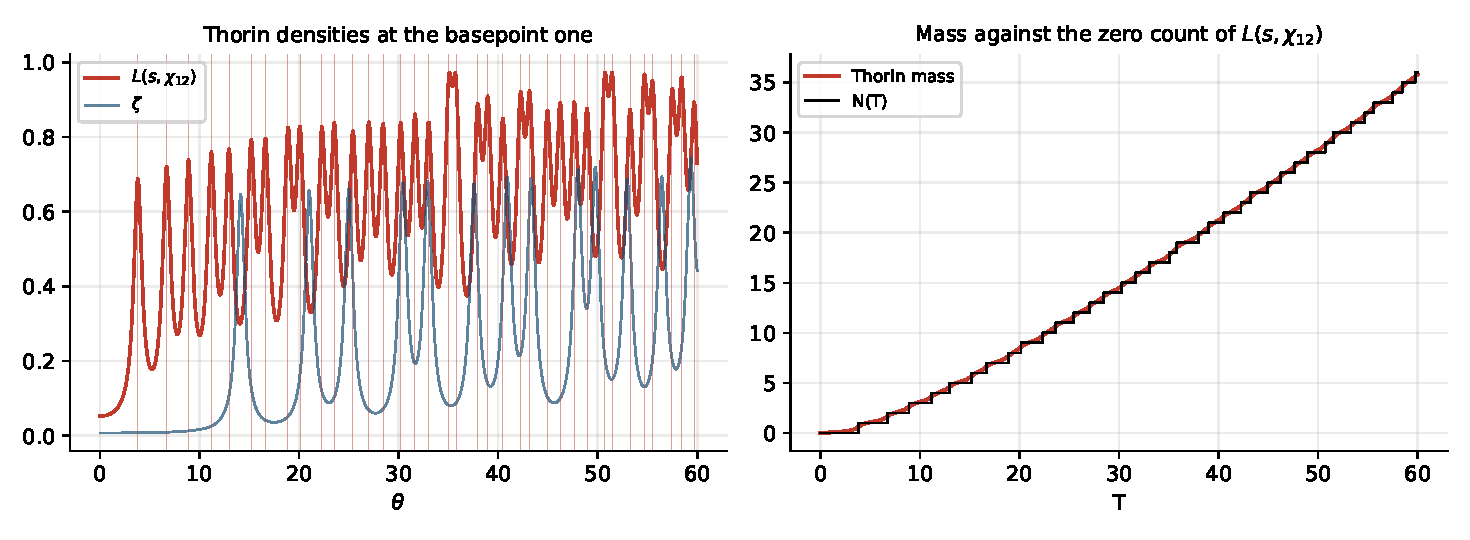
\includegraphics[width=\textwidth]{fig/bp1eta_density.pdf}
\caption{Left: the Thorin densities at the basepoint one for $L(s,\chi_{12})$ and for $\zeta$ on $[0,60]$, with the ordinates of the zeros of $L(s,\chi_{12})$ (vertical lines). Right: the cumulative Thorin mass for $L(s,\chi_{12})$ against its zero count $N_{\chi_{12}}(T)$, written $N(T)$ in the plot. Drawn by \texttt{figs.py} of \texttt{basepoint\_one/eta}.}
\label{bp:eta:fig:density}
\end{figure}

\subsection{The L\'evy form without a pole, at and below the basepoint one}\label{bp:eta:sec:levy}

The L\'evy form of Proposition~\ref{bp:prop:levy} has an exact analogue at the basepoint one, with no pole to compensate and with prime atoms of both signs.

\begin{proposition}\label{bp:eta:prop:levy}
For $\re s>0$,
\[
\log\frac{\xi(1+s,\chi_{12})}{\xi(1,\chi_{12})}=b_1s+\int_0^\infty(e^{-sx}-1+sx)\,\Pi(dx),
\]
where, with $\Lambda_{\chi_{12}}(n)=\chi_{12}(n)\Lambda(n)$,
\[
\Pi(dx)=\frac{e^{-x}}{x(1-e^{-2x})}\,dx+\sum_{n\ge2}\frac{\Lambda_{\chi_{12}}(n)}{n\log n}\,\delta_{\log n}(dx),
\]
the prime sum converging conditionally, as a limit over $n\le X$.
\end{proposition}

\begin{proof}
Binet's formula \cite[\S5.9]{DLMF} for $\log\Gamma(\frac12+\frac s2)$, in the integrated form of the proof of Proposition~\ref{bp:prop:levy} with $a=\frac12$, gives the gamma density; the factor $(12/\pi)^{s/2}$ and the linear terms combine into $b_1$; and for $\re s>0$ the Euler product gives
\[
\log L(1+s,\chi_{12})=\sum_n\frac{\Lambda_{\chi_{12}}(n)}{n\log n}\,e^{-s\log n}.
\]
The linear coefficient is $-\sum_n\Lambda_{\chi_{12}}(n)/n=\frac{L'}L(1,\chi_{12})$, which converges by the prime number theorem for arithmetic progressions \cite[Chapter~20]{Davenport}, in the form $\psi(y,\chi_{12})=O(y\,e^{-c\sqrt{\log y}})$, where $\psi(y,\chi_{12})=\sum_{n\le y}\Lambda_{\chi_{12}}(n)$ is the Chebyshev function of $\chi_{12}$.
\end{proof}

The form differs from that of $\zeta$ in two ways. There is no pole, so no compensating measure: the prime atoms converge on their own at the basepoint one. And the measure is signed for a different reason. For $\zeta$ the gamma density minus the pole term $dx/x$ is negative beyond $x=0.281$ and the prime atoms are positive; here the gamma density $e^{-x}/(x(1-e^{-2x}))$ is positive everywhere and the atoms carry the sign of $\chi_{12}(n)$, the first negative atom being $-\frac15$ at $\log5$, with canonical weight $-\frac{\log5}5$ (Figure~\ref{bp:eta:fig:levy}, left). Table~\ref{bp:eta:tab:levy}, computed by \texttt{arith.py}, checks the form.

The tilted eta variable $V_1$, with moment generating function $\xi(1+s,\chi_{12})/\xi(1,\chi_{12})$, is not quasi infinitely divisible. Its positive and its negative atoms each have infinite total mass, since $\sum_{\chi_{12}(p)=1}1/p$ and $\sum_{\chi_{12}(p)=-1}1/p$ both diverge by Dirichlet's theorem, and they cancel only conditionally, so the argument of Proposition~\ref{sb:prop:qid}(3) applies with $\xi(1+s,\chi_{12})$ in place of $\xi(1+s)$, as the discussion after its proof explains. Since an infinitely divisible law is quasi infinitely divisible, $V_1$ is not infinitely divisible either. At every basepoint $\alpha>1$, by contrast, $V_\alpha$ is quasi infinitely divisible: there the atoms of each sign have finite total mass, and the Euler product writes its characteristic function as that of an infinitely divisible gamma piece times a quotient of two compound Poisson characteristic functions.

\begin{table}[htbp]
\centering\small
\begin{tabular}{rrccccc}
\toprule
$s$ & $X$ & $b_1s$ & gamma piece & primes & total & exact\\
\midrule
0.5 & $10^5$ & 0.08254 & 0.121808 & $-0.082565$ & 0.121785 & 0.122329\\
0.5 & $10^7$ & 0.08254 & 0.121808 & $-0.081931$ & 0.122419 & 0.122329\\
1 & $10^7$ & 0.16508 & 0.409141 & $-0.254214$ & 0.320011 & 0.320099\\
2 & $10^7$ & 0.33017 & 1.270363 & $-0.689198$ & 0.911332 & 0.911001\\
\bottomrule
\end{tabular}
\caption{The L\'evy form of Proposition~\ref{bp:eta:prop:levy} against $\log(\xi(1+s,\chi_{12})/\xi(1,\chi_{12}))$, with primes up to $X$. The prime piece stays of order one; there is nothing to cancel.}
\label{bp:eta:tab:levy}
\end{table}

The sine squared lemma in the form of Section~\ref{bp:sec:levy}, with $\int_0^\infty\log(1+s^2/\theta^2)\,d\theta=\pi s$, converts the L\'evy form, with $s=\sqrt u$, into
\[
v_1(\theta)=b_1+A(\theta)+Q(\theta),
\]
with
\[
A(\theta)=\tfrac12\big[\re\psi(\tfrac{1+i\theta}2)-\psi(\tfrac12)\big],\qquad Q(\theta)=\sum_n\frac{\Lambda_{\chi_{12}}(n)}n\,2\sin^2\Big(\frac{\theta\log n}2\Big).
\]
The drift becomes the stable one half factor $e^{-b_1\sqrt u}$, the gamma factor the smooth positive growth $A$, and the primes the oscillating $Q$, now without any divergent partner. With primes to $10^7$ the formula gives $2.16385$ at $\theta=\gamma_1$ against the exact $2.16427$, and $0.84633$ at $\theta=10$ against $0.84649$. Figure~\ref{bp:eta:fig:levy} (right) shows the three pieces: the prime piece ranges over both signs, and the positivity of the sum comes from the drift and the gamma factor, as Section~\ref{sec:ch16:sin2} found at the basepoint two.

\begin{figure}[htbp]
\centering
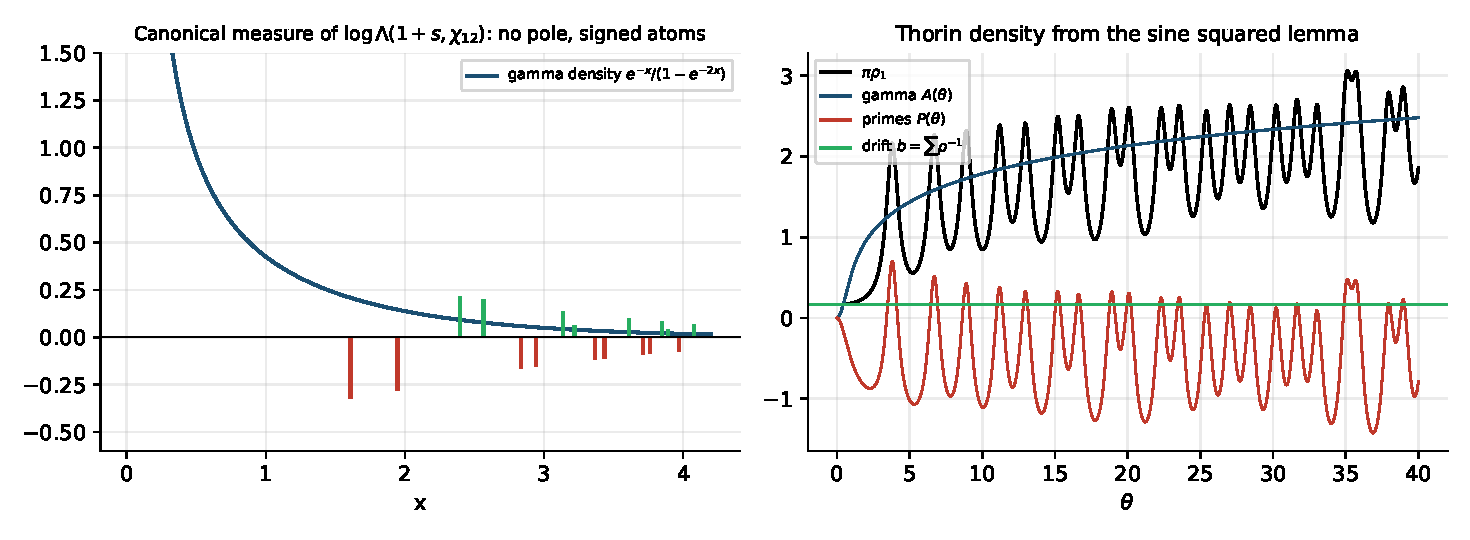
\includegraphics[width=\textwidth]{fig/bp1eta_levy.pdf}
\caption{Left: the canonical measure $x\Pi(dx)$ of $\log\xi(1+s,\chi_{12})$, written with $\Lambda(1+s,\chi_{12})$ in the plot: the positive gamma density $e^{-x}/(1-e^{-2x})$ and the prime atoms $\Lambda_{\chi_{12}}(n)/n$ at $\log n$, of both signs, the positive ones drawn upward and the negative ones downward; there is no pole. Right: $v_1(\theta)$ on $[0,40]$, written $\pi\rho_1$ in the plot, as the sum of the drift $b_1$, written $b$, the gamma piece $A(\theta)$ and the prime piece $Q(\theta)$, written $P(\theta)$ in the plot. Drawn by \texttt{figs.py} of \texttt{basepoint\_one/eta}.}
\label{bp:eta:fig:levy}
\end{figure}

\label{bp:eta:sec:below}Below the basepoint one, at $\alpha=1-\varepsilon$, the converted Thorin density is $\pi^{-1}$ times
\[
b_\alpha+A_\alpha(\theta)+\lim_{X\to\infty}\sum_{n\le X}\frac{\Lambda_{\chi_{12}}(n)}{n^\alpha}\,2\sin^2\Big(\frac{\theta\log n}2\Big),
\]
with $A_\alpha(\theta)=\frac12[\re\psi(\frac{\alpha+i\theta}2)-\psi(\frac\alpha2)]$. Exactly as for $\zeta$ in Proposition~\ref{bp:prop:below}, the limit exists and gives the positive Thorin density $v_\alpha/\pi$ when $L(s,\chi_{12})$ has no zeros with $\re s>\alpha'$ for some $\alpha'<\alpha$, and conversely its existence for $\re s>0$ in the L\'evy form forces the absence of zeros with $\re s>\alpha$. So the extension below one is, up to the boundary case, a zero free half plane for $L(s,\chi_{12})$, and at the centre it is GRH for $\chi_{12}$. The error at cutoff $X$ is given by the same explicit formula,
\[
\sum_\rho\Big[-\frac{X^{\rho-\alpha}}{\rho-\alpha}+\frac{X^{\rho-\alpha+i\theta}}{2(\rho-\alpha+i\theta)}+\frac{X^{\rho-\alpha-i\theta}}{2(\rho-\alpha-i\theta)}\Big]+O(X^{-\alpha}\log X),
\]
because $\psi(y,\chi_{12})=-\sum_\rho y^\rho/\rho+O(\log y)$ has no main term \cite[Chapter~19]{Davenport}.

The absence of a main term changes the numerics. For $\zeta$ the prime piece and the pole piece each grow like $X^{1-\alpha}/(1-\alpha)$ and must cancel; for $L(s,\chi_{12})$ the prime piece stays bounded. At $\alpha=0.6$, $\theta=\gamma_1$ and $X=10^7$ the prime piece is $6.07$, where for $\zeta$ the two pieces are about $1537$ each. Table~\ref{bp:eta:tab:below}, computed by \texttt{arith.py}, shows the errors, which decay like $X^{1/2-\alpha}$, and what remains after subtracting the explicit formula over the $297$ computed zeros. The correction removes most of the error at $\theta=\gamma_1$, by factors between $17$ and $2800$; at $\theta=10$, between zeros, it helps less, because $297$ zeros are fewer than the $1700$ used for $\zeta$ and the missing zeros above height $340$ dominate what remains. At the centre and the first ordinate the sum grows like $\log X$, taking the values $6.62$, $11.69$ and $16.77$ at $X=10^3$, $10^5$ and $10^7$: the atom $\delta_{\gamma_1}$ forming (Figure~\ref{bp:eta:fig:below}).

\begin{table}[htbp]
\centering\small
\begin{tabular}{cccccc}
\toprule
$\alpha$ & $\theta$ & $X$ & prime piece & error & error after zero correction\\
\midrule
1 & $\gamma_1$ & $10^5$ & 0.6964 & $-5.55\times10^{-3}$ & $4.2\times10^{-6}$\\
1 & $\gamma_1$ & $10^7$ & 0.7016 & $-4.15\times10^{-4}$ & $2.5\times10^{-5}$\\
0.75 & $\gamma_1$ & $10^5$ & 2.0933 & $-2.13\times10^{-1}$ & $1.4\times10^{-4}$\\
0.75 & $\gamma_1$ & $10^7$ & 2.2471 & $-5.92\times10^{-2}$ & $1.4\times10^{-3}$\\
0.6 & $\gamma_1$ & $10^5$ & 4.8292 & $-3.10$ & $1.1\times10^{-3}$\\
0.6 & $\gamma_1$ & $10^7$ & 6.0670 & $-1.86$ & $1.6\times10^{-2}$\\
0.6 & 10 & $10^7$ & $-2.4525$ & $-5.68\times10^{-2}$ & $2.6\times10^{-2}$\\
\bottomrule
\end{tabular}
\caption{The sine squared formula below the basepoint one for $L(s,\chi_{12})$, with primes up to $X$: the prime piece, the error against $v_\alpha(\theta)$, and the error left after subtracting the explicit formula over the $297$ computed zeros; $\gamma_1=3.8046276$.}
\label{bp:eta:tab:below}
\end{table}

\begin{figure}[htbp]
\centering
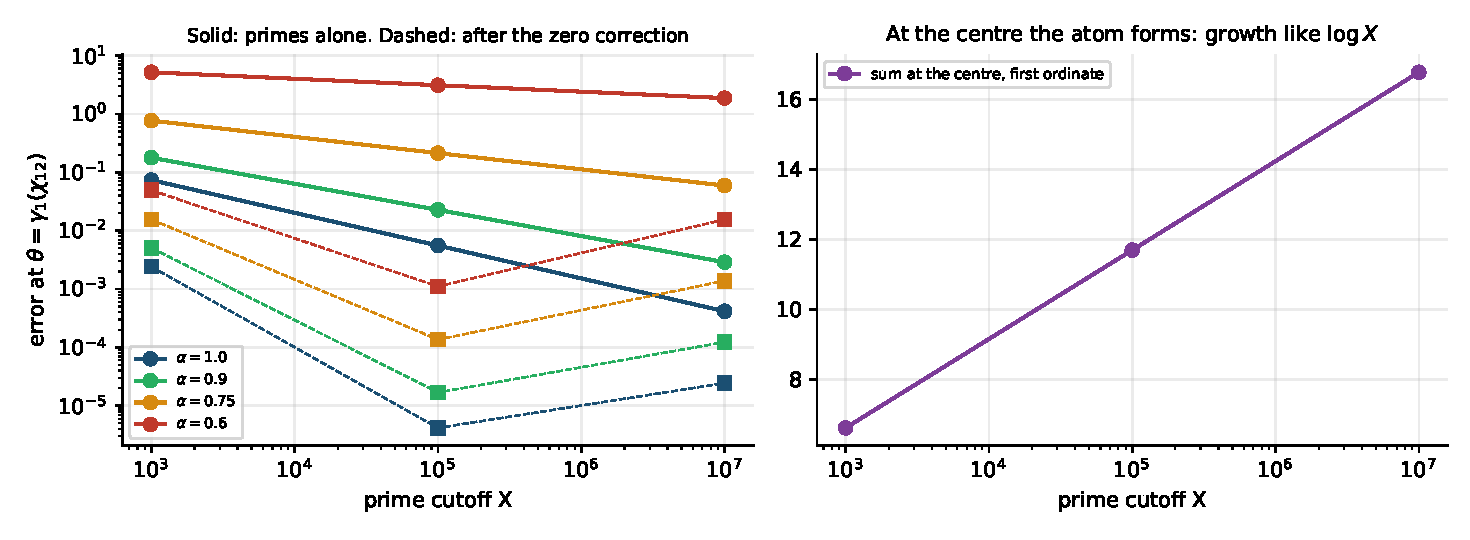
\includegraphics[width=\textwidth]{fig/bp1eta_below.pdf}
\caption{Left: absolute error at $\theta=\gamma_1=3.8046$ for $L(s,\chi_{12})$ against the prime cutoff $X$, for $\alpha=1$, $0.9$, $0.75$ and $0.6$, from primes alone (solid) and after the zero correction over $297$ zeros (dashed). Right: at the centre and the first ordinate the sum grows like $\log X$, the atom of the GRH measure forming. Drawn by \texttt{figs.py} of \texttt{basepoint\_one/eta}.}
\label{bp:eta:fig:below}
\end{figure}

\subsection{The hitting time and its boundary}\label{bp:eta:sec:hit}

The identity $(\frac12+\sqrt u)^2=\frac14+u+\sqrt u$ gives, as for $\zeta$,
\[
\varphi_1(u)=\frac{\varphi_{1/2}(\frac14+u+\sqrt u)}{\varphi_{1/2}(\frac14)},\qquad \varphi_{1/2}(u)=\frac{\xi(\frac12,\chi_{12})}{\xi(\frac12+\sqrt u,\chi_{12})} .
\]
Whenever the centre clock $\varphi_{1/2}$ is the Laplace transform of a probability law, and in particular under GRH for $\chi_{12}$, this reads $T_1\stackrel d=\widetilde T+H_{\widetilde T/\sqrt2}$, where $\widetilde T$ is the centre clock tilted by $e^{-T/4}$ and $H_a$ is the first passage time of Brownian motion to the level $a$, as in Theorem~\ref{bp:thm:sub}. Under GRH, $\widetilde T=\sum_ke_k/(\gamma_k^2+\frac14)$ with independent standard exponentials $e_k$; if the zeros are also simple, $\widetilde T$ is Kent's hitting time for a Krein string with spectrum $\{|\rho|^2\}$ \cite{Kent80}, and $T_1$ is the time for that string diffusion, run on the local time clock of a sticky Brownian motion, to reach its level, as in Corollary~\ref{bp:cor:kent}. As for $\zeta$, $T_1$ itself is not a hitting time of the kind in Kent's theorem, because its Thorin measure is absolutely continuous (Proposition~\ref{bp:eta:prop:thorin}).

We simulated $3\times10^5$ draws of $T_1$ with \texttt{hit.py}, taking $\widetilde T$ from this series under GRH: the terms of all $297$ computed zeros, and for the zeros above them a gamma variable matched to the tail sums of $p_1$ and $p_2$. The sample mean of $\widetilde T$ is $0.165108$ against $b_1=0.165083$, and the empirical Laplace transform agrees with $\varphi_1(u)=\xi(1,\chi_{12})/\xi(1+\sqrt u,\chi_{12})$ within $1.1$ standard errors at $u=0.1$, $0.5$, $1$, $5$ and $20$ (for instance $0.725800\pm0.000440$ against $0.726077$ at $u=1$, and $0.042364\pm0.000101$ against $0.042340$ at $u=20$).

We computed the Brownian boundary $b(t)$ whose crossing time has the law of $T_1$ from the Volterra equation \eqref{eq:ch19:volterra}, with the distribution function from Talbot inversion for $t<0.12$ and, under GRH as above, from the subordination representation beyond, and the complementary form of the equation once the survival probability falls below one half; \texttt{hit.py} solves it and \texttt{hit2.py} adds the tangent boundary and the checks. The time scale is about seven times that of $\zeta$, the ratio of the means of the two centre clocks. In the small time zone the boundary starts at the reflection level $1.008$ at $t=0.036$ and falls to $0.611$ at $t=0.08$; through the bulk it falls to $0.400$ at $t=0.12$ and $0.127$ at $t=0.2$, where the survival probability is one half; the tangent approximation agrees to $10^{-3}$ at $t=0.08$ and $5\times10^{-3}$ at $t=0.12$, then drifts, to $0.102$ at $t=0.2$. In the right tail the exact boundary flattens at $-0.2747$ ($-0.26030$ at $t=1$, $-0.27461$ at $t=100$, $-0.27471$ at $t=1000$), the Brownian form of the stable one half tail. The tangent approximation overshoots, to $-0.370$ at $t=0.4$ against the exact $-0.166$, and has no solution beyond $t=1.83$, for the reason explained in Section~\ref{bp:sec:rs1}: it cannot represent survivors that have wandered below the boundary.

Wald's identity fails in the same way as for $\zeta$, with the same proviso. The boundary is continuous and, as computed, bounded up to $t=1000$; if it is bounded on $[1,\infty)$, which here too is observed, not proved, Lemma~\ref{bp:lem:wald} and the stable tail give $\E\,b(T_1)=b_1/\sqrt2=\sum_\rho\rho^{-1}/\sqrt2=0.116732$; integrating the computed boundary against the law of $T_1$ gives $0.116749$. We simulated $1.5\times10^5$ Brownian paths against the exact boundary on $[0,5]$. Their survival function is within Kolmogorov distance $0.0014$ of the exact one (Figure~\ref{bp:eta:fig:hit}), and the simulated depth of the survivors below the boundary, $\E[(b(t)-B_t)\mathbf 1\{H_b>t\}]$, which tends to $\E\,b(T_1)$ by optional stopping, is $0.119$, $0.118$ and $0.118$ at $t=1$, $2$ and $5$.

\begin{figure}[htbp]
\centering
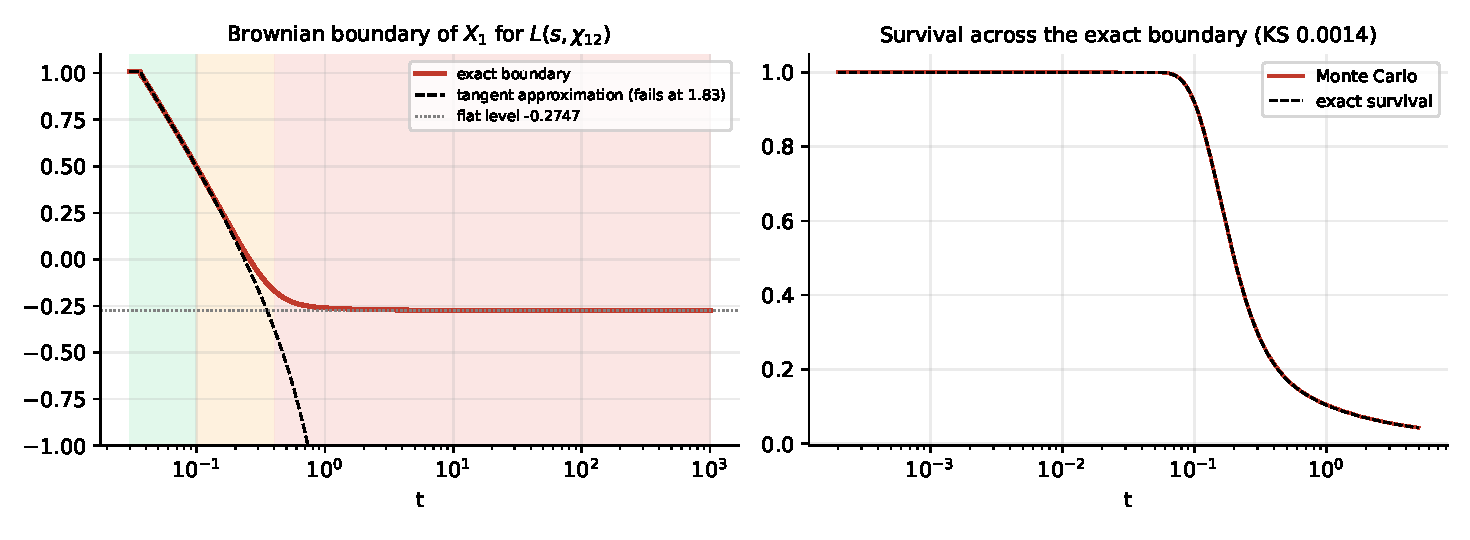
\includegraphics[width=\textwidth]{fig/bp1eta_hit.pdf}
\caption{Left: the exact Brownian boundary of $T_1$ for $L(s,\chi_{12})$, written $X_1$ in the plot, over the three zones of Section~\ref{sec:ch19:zones} (shaded), the tangent approximation, which fails at $t=1.83$, and the flat level $-0.2747$. Right: survival of $1.5\times10^5$ simulated Brownian paths across the exact boundary against the exact survival function; the Kolmogorov distance is $0.0014$. Drawn by \texttt{figs.py} of \texttt{basepoint\_one/eta}.}
\label{bp:eta:fig:hit}
\end{figure}

\subsection{The two examples compared}\label{bp:sec:compare}

Table~\ref{bp:eta:tab:cmp} sets the two basepoint one examples side by side. Structurally the eta case is the cleaner of the two: its kernel is a positive product, it has no pole, its L\'evy form converges at the basepoint one without compensation, and below the basepoint one its prime sums stay bounded, so the computation is far better conditioned. Nothing essential becomes easier, however. The negativity that $\zeta$ concentrates in the pole piece is carried here by the signs of $\chi_{12}(p)$; the extension of the L\'evy form below the line $\re s=1$ is equivalent to a zero free half plane for $L(s,\chi_{12})$; and, under GRH for $\chi_{12}$, the probabilistic picture is the same, with every constant scaled by the denser zeros: a stable one half subordination of the centre clock and, as computed, a boundary that flattens and, if it stays bounded, a Wald defect equal to $\sum_\rho\rho^{-1}/\sqrt2$.

\begin{table}[htbp]
\centering\small
\begin{tabular}{p{0.42\textwidth}p{0.26\textwidth}p{0.22\textwidth}}
\toprule
 & $\zeta$ & $L(s,\chi_{12})$\\
\midrule
kernel & theta series & $\eta(ix)$, a positive\newline product\\
pole & at $s=1$ & none\\
first zero & 14.134725 & 3.804628\\
drift $b_1=\sum_\rho\rho^{-1}$ & 0.0230957 & 0.1650833\\
tail constant $b_1/\sqrt\pi$ & 0.01303 & 0.09314\\
mean of the centre clock $\sum_ka_k^{-1}$ & 0.0231050 & 0.1664618\\
L\'evy measure, continuous part & gamma minus pole,\newline negative beyond $0.281$ & gamma only, positive\\
L\'evy measure, prime atoms & all positive & signs of $\chi_{12}(n)$\\
compensation at $\alpha=1$ & primes against $dx/x$\newline (prime number theorem) & none needed\\
prime piece at $\alpha=0.6$, $X=10^7$, $\theta=\gamma_1$ & about 1537,\newline cancelled by the pole & 6.07\\
flat level of the exact boundary & $-0.19277$ & $-0.27471$\\
$\E\,b(T_1)=b_1/\sqrt2$ & 0.016331 & 0.116732\\
tangent approximation fails at & $t=0.091$ & $t=1.83$\\
\bottomrule
\end{tabular}
\caption{The two basepoint one examples side by side: the reciprocal Xi function of Chapter~\ref{chap:basepoint} and the reciprocal completed $L$ function of $\chi_{12}$ of this section.}
\label{bp:eta:tab:cmp}
\end{table}

The comparison also closes the study of the basepoint one begun in Chapter~\ref{chap:basepoint}, and it confirms the two conclusions that fix the shape of the path to RH. First, at the basepoint one the constructions for the reciprocal Xi function are, with two exceptions, unconditional and explicit: the Thorin measure is the Poisson smoothing of the zeros, the L\'evy form comes from the primes, the gamma factor and the pole, the sine squared lemma converts one into the other with the drift $\sum_\rho\rho^{-1}$ becoming a stable one half factor, and the shifted clock is a subordinated hitting time whose Brownian boundary, as computed, becomes flat. The exceptions are the Krein string representation of Corollary~\ref{bp:cor:kent}, which assumes RH and simple zeros, and the Wald defect $\sum_\rho\rho^{-1}/\sqrt2$: Lemma~\ref{bp:lem:wald} gives it for a boundary bounded at infinity, and the boundedness of the computed boundary is observed, not proved. Second, below the basepoint one each positive statement for $\zeta$ holds, up to the boundary case, exactly when no zero lies to the right of the line $\re s=\alpha$: the convergence of the compensated L\'evy form, the GGC property of $T_\alpha$, the extended GGC property of the normal scale mixture, and the completeness in $L^1$ of the translates of the tilted P\'olya kernels on every line to the right of $\alpha$ (Propositions~\ref{bp:prop:below} and \ref{wr:prop:wiener}, Theorems~\ref{bp:thm:alpha} and \ref{sm:thm:strip}). The eta example shows that the pole changes how the prime sums converge, not where they stop.

The step that none of these constructions supplies is positivity of the Thorin measure at every height at a single basepoint $\alpha<1$, that is, the GGC property of $T_\alpha$, which by Theorem~\ref{thm:poisson} is a new zero free half plane, and then all the way to the centre. The variable $T_\alpha=\sigma^{(\alpha)}_{\widetilde T_\alpha}$ of Theorem~\ref{bp:thm:alpha} exists for every $\alpha>\frac12$ with no hypothesis, so only its GGC property is conditional; as $\alpha\downarrow\frac12$ the subordinator tends to pure drift, and the positivity must be supplied by the zeros themselves. Reaching any single $\alpha<1$ is step~7 of the path in Table~\ref{tab:ch25:path}, which the results of Sato and Bondesson do not reach either (Section~\ref{sb:sec:cannot}); for the methods of this book the basepoint one is where the path leaves the region of theorems. The half plane $\re s>\frac78$ announced in October 2026 for $\zeta$ and every Dirichlet $L$ function, $L(s,\chi_{12})$ included, would move that boundary to $\frac78$ by arithmetic from outside the book (Section~\ref{sec:ch25:open}).
